% Options for packages loaded elsewhere
\PassOptionsToPackage{unicode}{hyperref}
\PassOptionsToPackage{hyphens}{url}
%
\documentclass[
  ,man,floatsintext]{apa6}
\usepackage{amsmath,amssymb}
\usepackage{iftex}
\ifPDFTeX
  \usepackage[T1]{fontenc}
  \usepackage[utf8]{inputenc}
  \usepackage{textcomp} % provide euro and other symbols
\else % if luatex or xetex
  \usepackage{unicode-math} % this also loads fontspec
  \defaultfontfeatures{Scale=MatchLowercase}
  \defaultfontfeatures[\rmfamily]{Ligatures=TeX,Scale=1}
\fi
\usepackage{lmodern}
\ifPDFTeX\else
  % xetex/luatex font selection
\fi
% Use upquote if available, for straight quotes in verbatim environments
\IfFileExists{upquote.sty}{\usepackage{upquote}}{}
\IfFileExists{microtype.sty}{% use microtype if available
  \usepackage[]{microtype}
  \UseMicrotypeSet[protrusion]{basicmath} % disable protrusion for tt fonts
}{}
\makeatletter
\@ifundefined{KOMAClassName}{% if non-KOMA class
  \IfFileExists{parskip.sty}{%
    \usepackage{parskip}
  }{% else
    \setlength{\parindent}{0pt}
    \setlength{\parskip}{6pt plus 2pt minus 1pt}}
}{% if KOMA class
  \KOMAoptions{parskip=half}}
\makeatother
\usepackage{xcolor}
\usepackage{color}
\usepackage{fancyvrb}
\newcommand{\VerbBar}{|}
\newcommand{\VERB}{\Verb[commandchars=\\\{\}]}
\DefineVerbatimEnvironment{Highlighting}{Verbatim}{commandchars=\\\{\}}
% Add ',fontsize=\small' for more characters per line
\usepackage{framed}
\definecolor{shadecolor}{RGB}{248,248,248}
\newenvironment{Shaded}{\begin{snugshade}}{\end{snugshade}}
\newcommand{\AlertTok}[1]{\textcolor[rgb]{0.94,0.16,0.16}{#1}}
\newcommand{\AnnotationTok}[1]{\textcolor[rgb]{0.56,0.35,0.01}{\textbf{\textit{#1}}}}
\newcommand{\AttributeTok}[1]{\textcolor[rgb]{0.13,0.29,0.53}{#1}}
\newcommand{\BaseNTok}[1]{\textcolor[rgb]{0.00,0.00,0.81}{#1}}
\newcommand{\BuiltInTok}[1]{#1}
\newcommand{\CharTok}[1]{\textcolor[rgb]{0.31,0.60,0.02}{#1}}
\newcommand{\CommentTok}[1]{\textcolor[rgb]{0.56,0.35,0.01}{\textit{#1}}}
\newcommand{\CommentVarTok}[1]{\textcolor[rgb]{0.56,0.35,0.01}{\textbf{\textit{#1}}}}
\newcommand{\ConstantTok}[1]{\textcolor[rgb]{0.56,0.35,0.01}{#1}}
\newcommand{\ControlFlowTok}[1]{\textcolor[rgb]{0.13,0.29,0.53}{\textbf{#1}}}
\newcommand{\DataTypeTok}[1]{\textcolor[rgb]{0.13,0.29,0.53}{#1}}
\newcommand{\DecValTok}[1]{\textcolor[rgb]{0.00,0.00,0.81}{#1}}
\newcommand{\DocumentationTok}[1]{\textcolor[rgb]{0.56,0.35,0.01}{\textbf{\textit{#1}}}}
\newcommand{\ErrorTok}[1]{\textcolor[rgb]{0.64,0.00,0.00}{\textbf{#1}}}
\newcommand{\ExtensionTok}[1]{#1}
\newcommand{\FloatTok}[1]{\textcolor[rgb]{0.00,0.00,0.81}{#1}}
\newcommand{\FunctionTok}[1]{\textcolor[rgb]{0.13,0.29,0.53}{\textbf{#1}}}
\newcommand{\ImportTok}[1]{#1}
\newcommand{\InformationTok}[1]{\textcolor[rgb]{0.56,0.35,0.01}{\textbf{\textit{#1}}}}
\newcommand{\KeywordTok}[1]{\textcolor[rgb]{0.13,0.29,0.53}{\textbf{#1}}}
\newcommand{\NormalTok}[1]{#1}
\newcommand{\OperatorTok}[1]{\textcolor[rgb]{0.81,0.36,0.00}{\textbf{#1}}}
\newcommand{\OtherTok}[1]{\textcolor[rgb]{0.56,0.35,0.01}{#1}}
\newcommand{\PreprocessorTok}[1]{\textcolor[rgb]{0.56,0.35,0.01}{\textit{#1}}}
\newcommand{\RegionMarkerTok}[1]{#1}
\newcommand{\SpecialCharTok}[1]{\textcolor[rgb]{0.81,0.36,0.00}{\textbf{#1}}}
\newcommand{\SpecialStringTok}[1]{\textcolor[rgb]{0.31,0.60,0.02}{#1}}
\newcommand{\StringTok}[1]{\textcolor[rgb]{0.31,0.60,0.02}{#1}}
\newcommand{\VariableTok}[1]{\textcolor[rgb]{0.00,0.00,0.00}{#1}}
\newcommand{\VerbatimStringTok}[1]{\textcolor[rgb]{0.31,0.60,0.02}{#1}}
\newcommand{\WarningTok}[1]{\textcolor[rgb]{0.56,0.35,0.01}{\textbf{\textit{#1}}}}
\usepackage{graphicx}
\makeatletter
\def\maxwidth{\ifdim\Gin@nat@width>\linewidth\linewidth\else\Gin@nat@width\fi}
\def\maxheight{\ifdim\Gin@nat@height>\textheight\textheight\else\Gin@nat@height\fi}
\makeatother
% Scale images if necessary, so that they will not overflow the page
% margins by default, and it is still possible to overwrite the defaults
% using explicit options in \includegraphics[width, height, ...]{}
\setkeys{Gin}{width=\maxwidth,height=\maxheight,keepaspectratio}
% Set default figure placement to htbp
\makeatletter
\def\fps@figure{htbp}
\makeatother
\setlength{\emergencystretch}{3em} % prevent overfull lines
\providecommand{\tightlist}{%
  \setlength{\itemsep}{0pt}\setlength{\parskip}{0pt}}
\setcounter{secnumdepth}{-\maxdimen} % remove section numbering
% Make \paragraph and \subparagraph free-standing
\makeatletter
\ifx\paragraph\undefined\else
  \let\oldparagraph\paragraph
  \renewcommand{\paragraph}{
    \@ifstar
      \xxxParagraphStar
      \xxxParagraphNoStar
  }
  \newcommand{\xxxParagraphStar}[1]{\oldparagraph*{#1}\mbox{}}
  \newcommand{\xxxParagraphNoStar}[1]{\oldparagraph{#1}\mbox{}}
\fi
\ifx\subparagraph\undefined\else
  \let\oldsubparagraph\subparagraph
  \renewcommand{\subparagraph}{
    \@ifstar
      \xxxSubParagraphStar
      \xxxSubParagraphNoStar
  }
  \newcommand{\xxxSubParagraphStar}[1]{\oldsubparagraph*{#1}\mbox{}}
  \newcommand{\xxxSubParagraphNoStar}[1]{\oldsubparagraph{#1}\mbox{}}
\fi
\makeatother
% definitions for citeproc citations
\NewDocumentCommand\citeproctext{}{}
\NewDocumentCommand\citeproc{mm}{%
  \begingroup\def\citeproctext{#2}\cite{#1}\endgroup}
\makeatletter
 % allow citations to break across lines
 \let\@cite@ofmt\@firstofone
 % avoid brackets around text for \cite:
 \def\@biblabel#1{}
 \def\@cite#1#2{{#1\if@tempswa , #2\fi}}
\makeatother
\newlength{\cslhangindent}
\setlength{\cslhangindent}{1.5em}
\newlength{\csllabelwidth}
\setlength{\csllabelwidth}{3em}
\newenvironment{CSLReferences}[2] % #1 hanging-indent, #2 entry-spacing
 {\begin{list}{}{%
  \setlength{\itemindent}{0pt}
  \setlength{\leftmargin}{0pt}
  \setlength{\parsep}{0pt}
  % turn on hanging indent if param 1 is 1
  \ifodd #1
   \setlength{\leftmargin}{\cslhangindent}
   \setlength{\itemindent}{-1\cslhangindent}
  \fi
  % set entry spacing
  \setlength{\itemsep}{#2\baselineskip}}}
 {\end{list}}
\usepackage{calc}
\newcommand{\CSLBlock}[1]{\hfill\break\parbox[t]{\linewidth}{\strut\ignorespaces#1\strut}}
\newcommand{\CSLLeftMargin}[1]{\parbox[t]{\csllabelwidth}{\strut#1\strut}}
\newcommand{\CSLRightInline}[1]{\parbox[t]{\linewidth - \csllabelwidth}{\strut#1\strut}}
\newcommand{\CSLIndent}[1]{\hspace{\cslhangindent}#1}
\ifLuaTeX
\usepackage[bidi=basic]{babel}
\else
\usepackage[bidi=default]{babel}
\fi
\babelprovide[main,import]{english}
% get rid of language-specific shorthands (see #6817):
\let\LanguageShortHands\languageshorthands
\def\languageshorthands#1{}
% Manuscript styling
\usepackage{upgreek}
\captionsetup{font=singlespacing,justification=justified}

% Table formatting
\usepackage{longtable}
\usepackage{lscape}
% \usepackage[counterclockwise]{rotating}   % Landscape page setup for large tables
\usepackage{multirow}		% Table styling
\usepackage{tabularx}		% Control Column width
\usepackage[flushleft]{threeparttable}	% Allows for three part tables with a specified notes section
\usepackage{threeparttablex}            % Lets threeparttable work with longtable

% Create new environments so endfloat can handle them
% \newenvironment{ltable}
%   {\begin{landscape}\centering\begin{threeparttable}}
%   {\end{threeparttable}\end{landscape}}
\newenvironment{lltable}{\begin{landscape}\centering\begin{ThreePartTable}}{\end{ThreePartTable}\end{landscape}}

% Enables adjusting longtable caption width to table width
% Solution found at http://golatex.de/longtable-mit-caption-so-breit-wie-die-tabelle-t15767.html
\makeatletter
\newcommand\LastLTentrywidth{1em}
\newlength\longtablewidth
\setlength{\longtablewidth}{1in}
\newcommand{\getlongtablewidth}{\begingroup \ifcsname LT@\roman{LT@tables}\endcsname \global\longtablewidth=0pt \renewcommand{\LT@entry}[2]{\global\advance\longtablewidth by ##2\relax\gdef\LastLTentrywidth{##2}}\@nameuse{LT@\roman{LT@tables}} \fi \endgroup}

% \setlength{\parindent}{0.5in}
% \setlength{\parskip}{0pt plus 0pt minus 0pt}

% Overwrite redefinition of paragraph and subparagraph by the default LaTeX template
% See https://github.com/crsh/papaja/issues/292
\makeatletter
\renewcommand{\paragraph}{\@startsection{paragraph}{4}{\parindent}%
  {0\baselineskip \@plus 0.2ex \@minus 0.2ex}%
  {-1em}%
  {\normalfont\normalsize\bfseries\itshape\typesectitle}}

\renewcommand{\subparagraph}[1]{\@startsection{subparagraph}{5}{1em}%
  {0\baselineskip \@plus 0.2ex \@minus 0.2ex}%
  {-\z@\relax}%
  {\normalfont\normalsize\itshape\hspace{\parindent}{#1}\textit{\addperi}}{\relax}}
\makeatother

\makeatletter
\usepackage{etoolbox}
\patchcmd{\maketitle}
  {\section{\normalfont\normalsize\abstractname}}
  {\section*{\normalfont\normalsize\abstractname}}
  {}{\typeout{Failed to patch abstract.}}
\patchcmd{\maketitle}
  {\section{\protect\normalfont{\@title}}}
  {\section*{\protect\normalfont{\@title}}}
  {}{\typeout{Failed to patch title.}}
\makeatother

\usepackage{xpatch}
\makeatletter
\xapptocmd\appendix
  {\xapptocmd\section
    {\addcontentsline{toc}{section}{\appendixname\ifoneappendix\else~\theappendix\fi: #1}}
    {}{\InnerPatchFailed}%
  }
{}{\PatchFailed}
\makeatother
\keywords{keywords\newline\indent Word count: X}
\usepackage{csquotes}
\usepackage[titles]{tocloft}
\cftpagenumbersoff{figure}
\renewcommand{\cftfigpresnum}{\itshape\figurename\enspace}
\renewcommand{\cftfigaftersnum}{.\space}
\setlength{\cftfigindent}{0pt}
\setlength{\cftafterloftitleskip}{0pt}
\settowidth{\cftfignumwidth}{Figure 10.\qquad}
\cftpagenumbersoff{table}
\renewcommand{\cfttabpresnum}{\itshape\tablename\enspace}
\renewcommand{\cfttabaftersnum}{.\space}
\setlength{\cfttabindent}{0pt}
\setlength{\cftafterloftitleskip}{0pt}
\settowidth{\cfttabnumwidth}{Table 10.\qquad}
\ifLuaTeX
  \usepackage{selnolig}  % disable illegal ligatures
\fi
\usepackage{bookmark}
\IfFileExists{xurl.sty}{\usepackage{xurl}}{} % add URL line breaks if available
\urlstyle{same}
\hypersetup{
  pdftitle={Variation of {[}v{]} in Cook Islands Māori},
  pdfauthor={Quartz ColvinRutgers University},
  pdflang={en-EN},
  pdfkeywords={keywords},
  hidelinks,
  pdfcreator={LaTeX via pandoc}}

\title{Variation of {[}v{]} in Cook Islands Māori}
\author{Quartz Colvin\textsuperscript{Rutgers University}}
\date{}


\shorttitle{Cook Islands Māori}

\affiliation{\phantom{0}}

\begin{document}
\maketitle

\section{1.0 Introduction}\label{introduction}

In this paper, we will do a statistical analysis of {[}v{]} across a sample of islands in Cook Islands Māori (CIM). It's known that in many dialects and other varieties of Māori, this phoneme can be realized as {[}w{]} or {[}v{]}. This paper aims to take a statistical approach to this generalization.

This paper has four sub-questions to investigate. First, how does w\textasciitilde v duration vary by island and second, how does intensity for these phonemes vary by island. The other two questions are about identifying information about the surface forms of w\textasciitilde v by island. Specifically, we will model f0 and f2 to determine whether certain islands have a voiced phoneme realized. Finally, the f2 model will help us determine which islands have higher rates of {[}w{]}s surfacing and which have more {[}v{]}s surfacing.

\subsection{1.1 Background (CIM)}\label{background-cim}

Cook Islands Māori is an Eastern Polynesian language classified as \emph{Vulnerable}. It is very closely related to Aotearoa Māori, but is definitely different from it.

It's known across both Aotearoa (NZ) Māori and CIM that some speakers regularly pronounce {[}v{]} as {[}w{]}, but it isn't clear to anyone who does this more and what conditions it.

\section{2.0 Methods}\label{methods}

\section{3.0 Data}\label{data}

This data set contains a lot of information, so we will need to tidy it and only keep the relevant data for the analysis. The following code chunk shows how the data was tidied and what was kept from the untidy data set. I don't show a preview of the untidy data set here because it had 17 columns and most of the columns will be taken out. In addition, it includes some metadata that I did not ask permission to share.

\begin{Shaded}
\begin{Highlighting}[]
\NormalTok{dat }\OtherTok{\textless{}{-}}\NormalTok{ untidy\_data }\SpecialCharTok{|\textgreater{}}
  \FunctionTok{drop\_na}\NormalTok{() }\SpecialCharTok{|\textgreater{}}   \CommentTok{\# remove rows that have NA values}
  \FunctionTok{filter}\NormalTok{(TextGridLabel }\SpecialCharTok{==} \StringTok{"v"}\NormalTok{) }\SpecialCharTok{|\textgreater{}}   \CommentTok{\# filter by \textquotesingle{}v\textquotesingle{} for analysis}
  \FunctionTok{pivot\_longer}\NormalTok{(      }\CommentTok{\# deal with all the f0 columns}
    \AttributeTok{cols =} \FunctionTok{c}\NormalTok{(}\StringTok{"f0\_20.point"}\NormalTok{, }
             \StringTok{"f0\_50.point"}\NormalTok{, }
             \StringTok{"f0\_80.point"}\NormalTok{),}
    \AttributeTok{names\_to =} \StringTok{"percent"}\NormalTok{,    }\CommentTok{\# names to \textquotesingle{}percent\textquotesingle{} column}
    \AttributeTok{values\_to =} \StringTok{"hz"}      \CommentTok{\# values to one column called \textquotesingle{}hz\textquotesingle{}}
\NormalTok{  ) }\SpecialCharTok{|\textgreater{}}
  \FunctionTok{arrange}\NormalTok{(island, Word) }\SpecialCharTok{|\textgreater{}}   \CommentTok{\# group by \textquotesingle{}island\textquotesingle{}, then \textquotesingle{}word\textquotesingle{}}
  \FunctionTok{select}\NormalTok{(island,      }\CommentTok{\# pick which columns I want and rename some}
         \AttributeTok{word =}\NormalTok{ Word, }
\NormalTok{         percent, hz, }\AttributeTok{f2 =}\NormalTok{ F2\_midpoint, duration, }
         \AttributeTok{intensity =}\NormalTok{ intensity\_midpoint) }\SpecialCharTok{|\textgreater{}}
  \FunctionTok{write\_csv}\NormalTok{(}\StringTok{"tidy\_cim.csv"}\NormalTok{)    }\CommentTok{\# put tidy data in new .csv}
\end{Highlighting}
\end{Shaded}

In the new data set, we need to fix the names that we've converted to values under `percent'. This is shown in the following code chunk.

\begin{Shaded}
\begin{Highlighting}[]
\CommentTok{\# fixing the original column names to only be the percent}
\CommentTok{\# since they are all values for f0}

\NormalTok{dat}\SpecialCharTok{$}\NormalTok{percent[dat}\SpecialCharTok{$}\NormalTok{percent }\SpecialCharTok{==} \StringTok{\textquotesingle{}f0\_20.point\textquotesingle{}}\NormalTok{] }\OtherTok{\textless{}{-}} \StringTok{"20"}

\NormalTok{dat}\SpecialCharTok{$}\NormalTok{percent[dat}\SpecialCharTok{$}\NormalTok{percent }\SpecialCharTok{==} \StringTok{\textquotesingle{}f0\_50.point\textquotesingle{}}\NormalTok{] }\OtherTok{\textless{}{-}} \StringTok{"50"}

\NormalTok{dat}\SpecialCharTok{$}\NormalTok{percent[dat}\SpecialCharTok{$}\NormalTok{percent }\SpecialCharTok{==} \StringTok{\textquotesingle{}f0\_80.point\textquotesingle{}}\NormalTok{] }\OtherTok{\textless{}{-}} \StringTok{"80"}
\end{Highlighting}
\end{Shaded}

Now that we have tidied this data set, here is a preview showing what it looks like.

\begin{tabular}{l|l|l|r|r|r|r}
\hline
island & word & percent & hz & f2 & duration & intensity\\
\hline
Atiu & ava & 20 & 128.5916 & 964.3925 & 0.08 & 54.08202\\
\hline
Atiu & ava & 50 & 127.0908 & 964.3925 & 0.08 & 54.08202\\
\hline
Atiu & ava & 80 & 127.4540 & 964.3925 & 0.08 & 54.08202\\
\hline
Atiu & ava & 20 & 160.6464 & 950.2333 & 0.07 & 58.06061\\
\hline
Atiu & ava & 50 & 157.4397 & 950.2333 & 0.07 & 58.06061\\
\hline
Atiu & ava & 80 & 158.2820 & 950.2333 & 0.07 & 58.06061\\
\hline
\end{tabular}

There are many more rows than this, but if all rows were included, it would be too long of a table to show here. To explain the column names, ``Percent'' refers to the 20\% 50\% and 80\% marks of the phoneme's total duration and ``HZ'' refers to the f0 measurement (in Hz) at that mark. ``f2'' is formant 2 measured in Hz at the midpoint of the phoneme. ``Duration'' is the total duration for the phoneme and ``Intensity'' is the intensity extracted from the midpoint of the phoneme.

\section{4.0 Analysis}\label{analysis}

This section readdresses the main questions about the w\textasciitilde v alternation. First, how does duration differ by island and second, how does intensity vary by island? Finally, do any islands have regular occurrence of {[}w{]} instead of {[}v{]} surfacing. For this final question, we will compare f0 and f2 separately.

Note that in all of my models, I did not control for where w\textasciitilde v occurs in the word, since I am looking at general frequency information and not doing a phonological analysis of specific environments in which {[}w{]} or {[}v{]} occurs more.

\subsection{4.1 Duration by island}\label{duration-by-island}

First, we compare the duration of {[}v{]} across the four islands. To do this, I will fit a \emph{linear model} below to track the relationship between the duration of w\textasciitilde v and which island a speaker is from. For this model, duration is the dependent variable and island is the independent or predictor variable.

Before we fit the model, we need to see if fitting a model for duration is appropriate. The visual qq-plot test for duration shows that we need to transform the values for duration in order to fit a model.

To normalize the duration variable, we need to log-transform the data. So, we make a new column where we apply `log()' to the `duration' column with 0.1 added to it, and then add the new column to the dataset. The following boxplot shows the normalized durations by island.

\begin{figure}
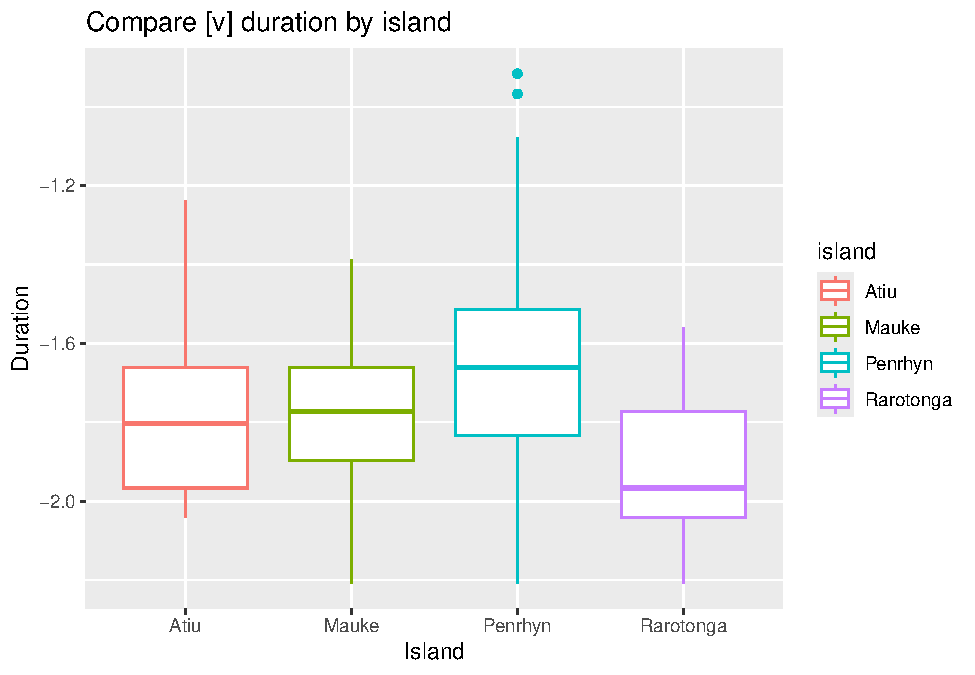
\includegraphics[width=0.75\linewidth]{cim_w_v_manuscript_files/figure-latex/print-mod1-1} \caption{ }\label{fig:print-mod1}
\end{figure}

A few things are visually clear from this comparative boxplot. Most obviously, Penrhyn had the largest range of w\textasciitilde v durations and Rarotonga had the smallest range. Rarotonga also had the lowest average duration for w\textasciitilde v and Penrhyn had the highest average duration. Interestingly, Mauke and Rarotonga didn't seem to have outliers in w\textasciitilde v durations, but Atiu and Penrhyn had a few outlier data points.

\subsection{4.2 Intensity by island}\label{intensity-by-island}

Next, in the same fashion we did to compare duration of {[}v{]} tokens, we can compare the intensity midpoints for the tokens across the islands. First we need to look at a qq-plot to see if fitting a model for intensity is an appropriate decision.

The qq-plot test showed that intensity \emph{is} normally distributed, so we can fit a model for intensity. Once again I fit a linear model for intensity (the dependent variable) by island (the predictor variable). The results are shown via a boxplot again.

\begin{figure}
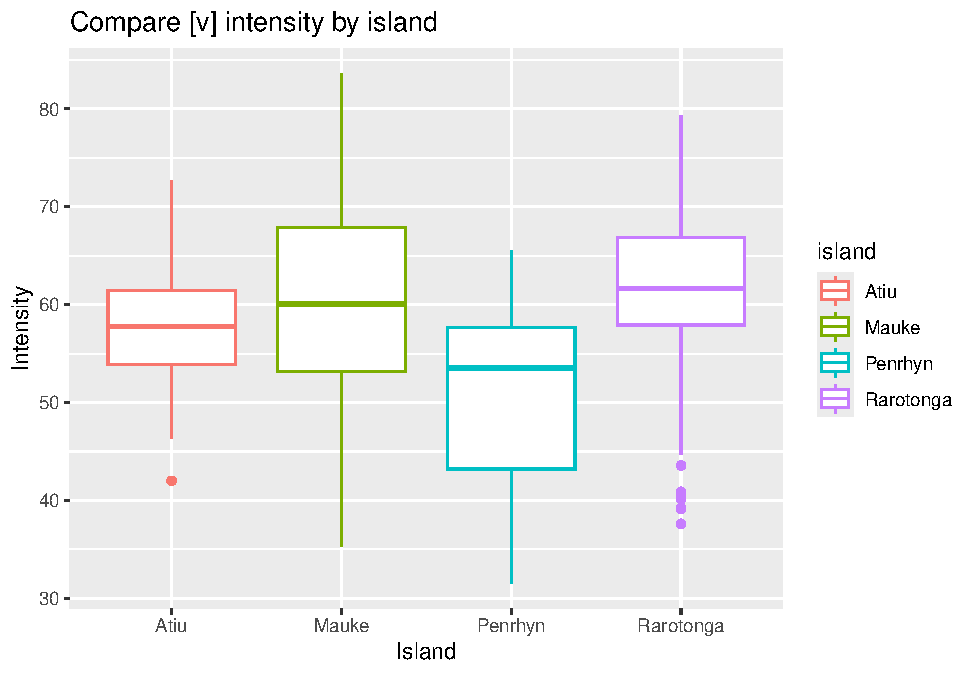
\includegraphics[width=0.75\linewidth]{cim_w_v_manuscript_files/figure-latex/print-mod2-1} \caption{ }\label{fig:print-mod2}
\end{figure}

Looking at the comparative boxplot, we can see how intensity midpoints vary across these four islands. The average intensity values were similar for all four, but Penrhyn had the lowest mean. These averages varied by less than 10, so they are quite similar. Mauke had the highest range for intensity midpoints, while Atiu had the smallest. Rarotonga had the most outliers and the other three islands had basically no outliers.

\subsection{4.3 Voicing by island}\label{voicing-by-island}

Now we can investigate how voicing of w\textasciitilde v varies by island. The f0 values used for this were extracted at the 20\%, 50\% and 80\% points of the duration of the target phoneme.

Again, we first need to check if fitting a model for this variable is appropriate. If we do another visual qq-plot test, we find that `Hz' is normally distributed and thus we can fit a model.

This time, I will show the model results in a scatterplot with a facet for each island. These plots show how F0 (measured in Hz) changes over the duration of the w\textasciitilde v tokens.

\begin{figure}
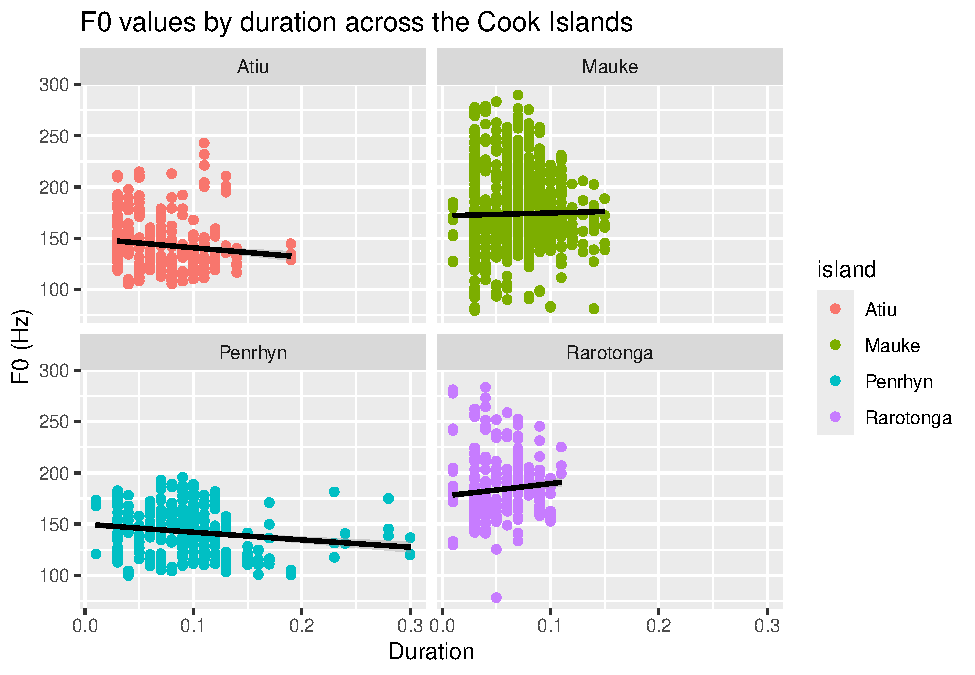
\includegraphics[width=0.75\linewidth]{cim_w_v_manuscript_files/figure-latex/print-modf0-1} \caption{ }\label{fig:print-modf0}
\end{figure}

As noted earlier, duration clearly differs between these four islands. The slopes for Atiu and Penrhyn show that over the duration of the phoneme, f0 decreases. This slope isn't steep, but it is present. Mauke and Rarotonga have upwards slopes, showing that over the duration of {[}v{]}, the f0 tends to increase. Rarotongan Māori has the sharpest increase in Hz over the duration of the phoneme.

Mauke is the only one that seems to \emph{regularly} have voiceless {[}w{]} in place of `v', but it also has the biggest overall range for f0 Hz. The other three islands typically have f0 values \textgreater{} 100 Hz, so these tokens are voiced.

In summary, it seems that f0 was not a good predictor for the {[}w{]} vs.~{[}v{]} question, but it did reveal that Mauke's {[}w{]} phoneme has a higher rate of voicelessness when it is realized.

\subsection{4.4 w\textasciitilde v distribution by island}\label{wv-distribution-by-island}

Finally, we can revisit the main question of this article: which islands have more {[}w{]} or more {[}v{]}? One of the primary acoustic differences between {[}w{]} and {[}v{]} is that {[}w{]} has a lower f2. Here, we define ``low f2'' as \textless850 Hz. To investigate this question, we will fit a model for f2 by island.

If we do a visual qq-plot test, we find that the raw data for f2 are \emph{not} normally distributed. Before we fit the model, we need to use `log()' to transform the data and put it in a new column like we did for duration.

\begin{figure}
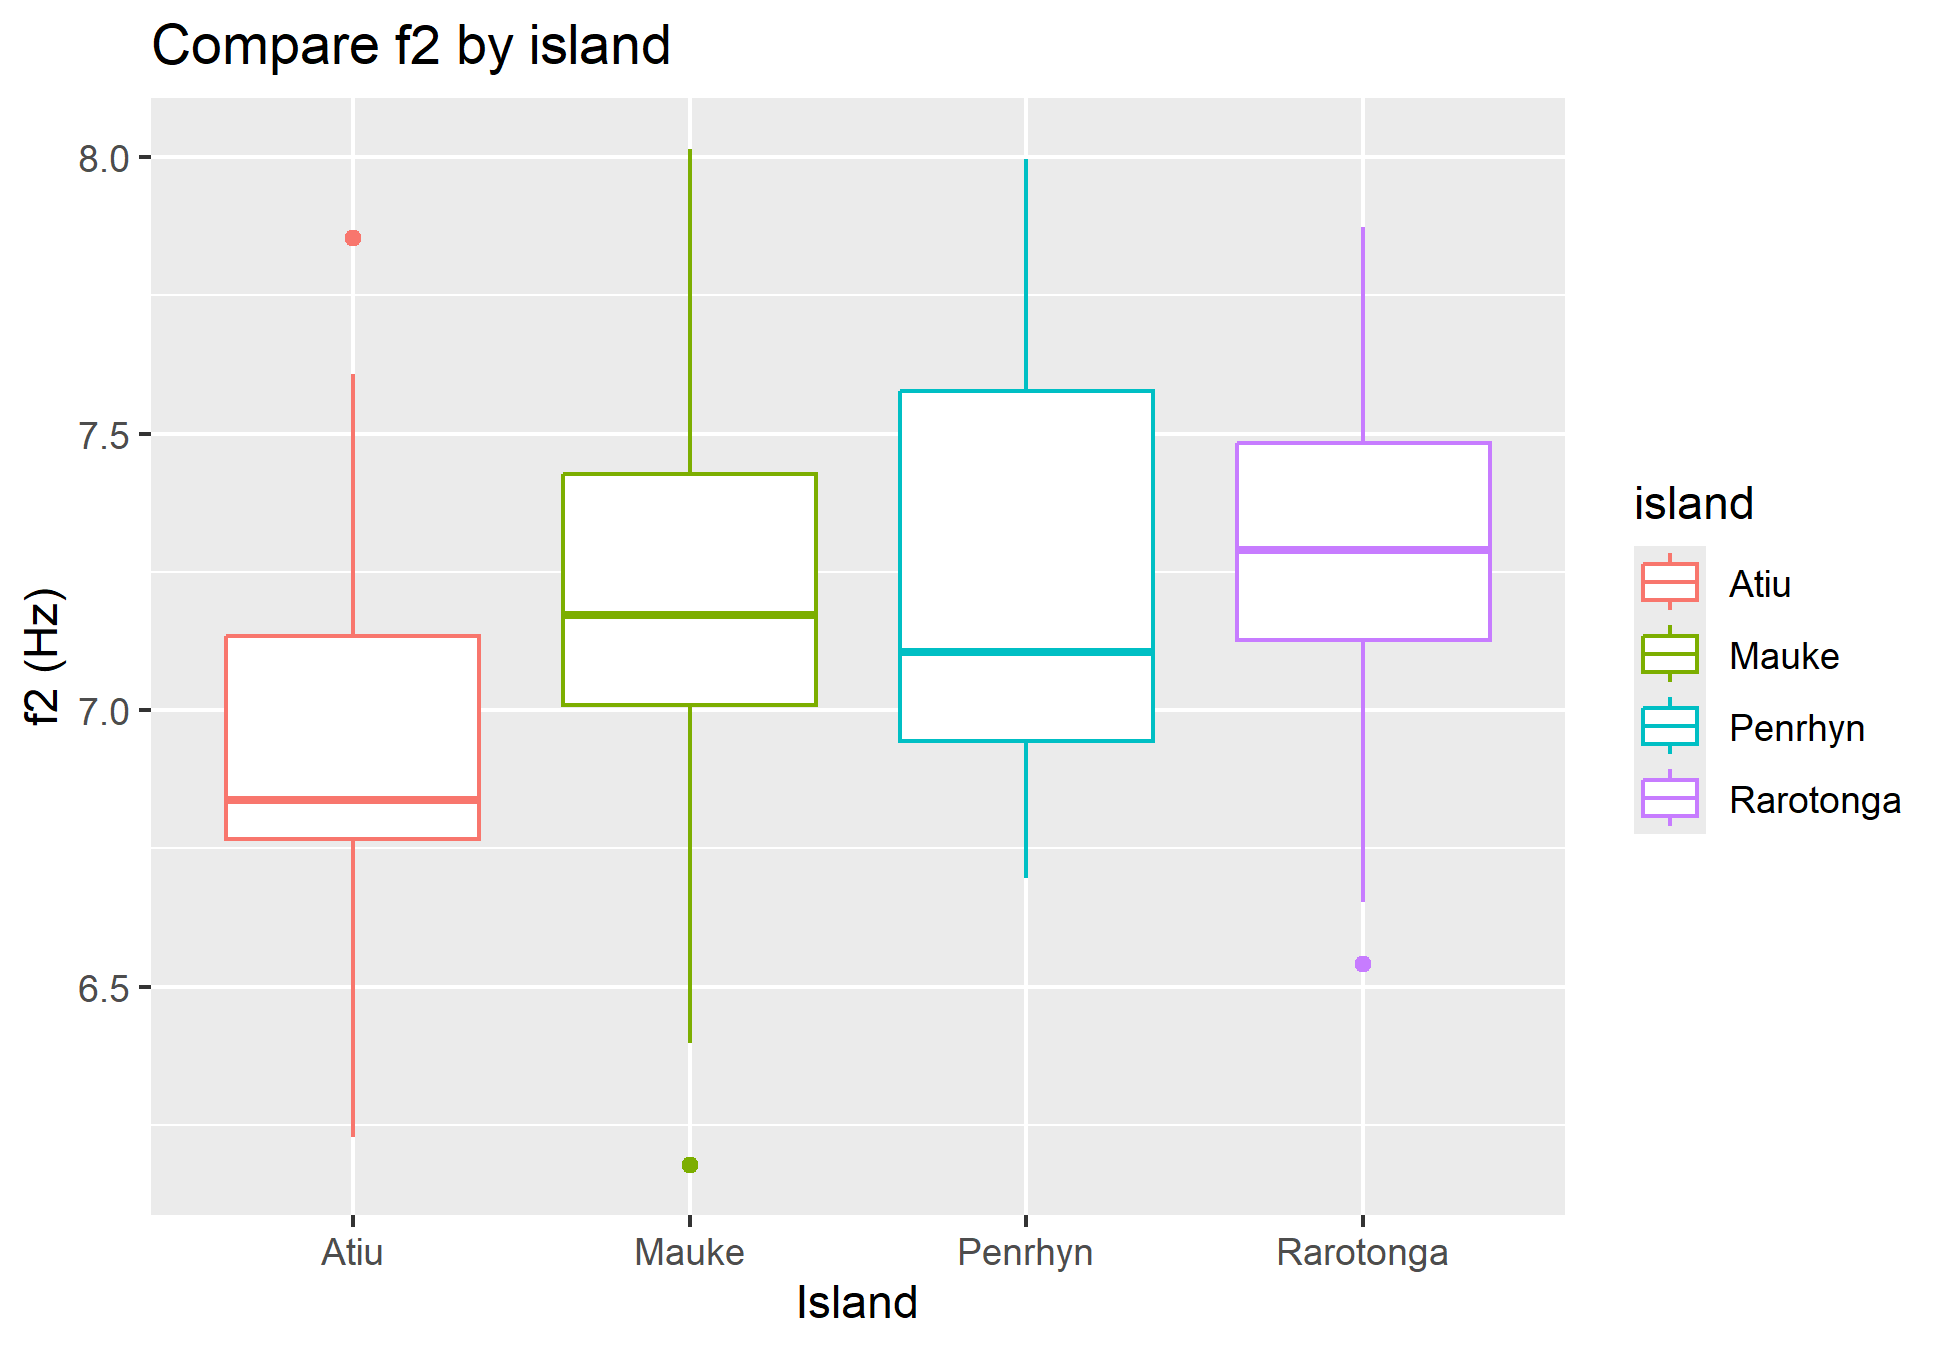
\includegraphics[width=0.75\linewidth]{cim_w_v_manuscript_files/figure-latex/print-plot-f2-1} \caption{ }\label{fig:print-plot-f2}
\end{figure}

Since we normalized the f2 values in the model, we also have to transform the cutoff point of 850 Hz by the same log transformation we did for the real f2 values. If we do this, the cutoff point in our model is 6.75.

Visually, all of these four islands have instances of {[}w{]}, and their means are all slightly (or much) higher than the cut-off point. Additionally, all of the islands except Penrhyn have \emph{many} tokens where `v' surfaces as {[}w{]}.

\section{5.0 Formal results}\label{formal-results}

To interpret the results of each model, we will do t-tests for the normalized versions of each model. If p \textless{} 0.05 then the difference is not random chance. For the t values, a larger t value indicates a greater difference between the means.

For \emph{normalized duration}, t=-408.11 and p-value \textless{} 2.2e-16, and there is a 95\% confidence interval. For \emph{intensity}, t=286.21, p-value \textless{} 2.2e-16 and there is a 95\% confidence interval. For \emph{hz} (f0), t=207.57, the p-value is \textless{} 2.2e-16, and we have a 95\% confidence interval. For \emph{normalized f2}, t=1060.9, p-value is \textless{} 2.2e-16 and we have a 95\% confidence interval.

All of these p-values are \textless{} 0.05, so duration, intensity, f0 (Hz column), and f2 are all statistically significant interactions with island. T values for duration and f2 were the furthest from 0, so these acoustic properties varied the most depending on which island a speaker was from.

I now want to pose the question of what percent of w\textasciitilde v surface as {[}w{]} and {[}v{]} for each island in the data, now that we have the values and a cutoff value for f2. This requires another bit of data transformation to calculate percentages. The first transformation step is adding a new column that says ``v'' if the value in log\_f2 is greater than the cutoff value, and outputs ``w'' if the value in the `log\_f2' column is lower than the cutoff value.

\begin{tabular}{l|l|l|l|l|l|l|l|l}
\hline
island & Atiu & Atiu & Mauke & Mauke & Penrhyn & Penrhyn & Rarotonga & Rarotonga\\
\hline
surface\_form & v & w & v & w & v & w & v & w\\
\hline
freq & 264 & 54 & 1005 & 42 & 327 & 6 & 303 & 6\\
\hline
\end{tabular}

I manually calculated the percentages of {[}w{]}s surfacing in each group (island). The percent of {[}w{]}s in Atiu was 16.98\%, 4.01\% for Mauke, 1.80\% for Penrhyn and 1.94\% for Rarotonga.

We can also transform the data in a similar way to calculate the percentages of {[}w{]} that are voiced in each island.

\begin{tabular}{l|l|l|l|l|l|l|l}
\hline
island & Atiu & Mauke & Mauke & Penrhyn & Penrhyn & Rarotonga & Rarotonga\\
\hline
voiceless\_w & 318 & 1023 & 24 & 332 & 1 & 308 & 1\\
\hline
\end{tabular}

The percentage of voiceless {[}w{]}s in Mauke was 2.29\%, for Penrhyn it was 0.30\% and for Rarotonga it was 0.32\%.

\subsection{5.1 Data analysis}\label{data-analysis}

I used R (Version 4.5.0; R Core Team, 2024) and the R-packages \emph{dplyr} (Version 1.1.4; Wickham, François, Henry, Müller, \& Vaughan, 2023), \emph{ds4ling} (Version 1.0; Casillas, 2025), \emph{forcats} (Version 1.0.0; Wickham, 2023a), \emph{ggplot2} (Version 3.5.2; Wickham, 2016), \emph{ggpubr} (Version 0.6.0; Kassambara, 2023), \emph{here} (Version 1.0.1; Müller, 2020), \emph{lme4} (Version 1.1.37; Bates, Mächler, Bolker, \& Walker, 2015), \emph{lmerTest} (Version 3.1.3; Kuznetsova, Brockhoff, \& Christensen, 2017), \emph{lubridate} (Version 1.9.4; Grolemund \& Wickham, 2011), \emph{Matrix} (Version 1.7.3; Bates, Maechler, \& Jagan, 2025), \emph{papaja} (Version 0.1.3; Aust \& Barth, 2024), \emph{purrr} (Version 1.0.4; Wickham \& Henry, 2025), \emph{readr} (Version 2.1.5; Wickham, Hester, \& Bryan, 2024), \emph{stringr} (Version 1.5.1; Wickham, 2023b), \emph{tibble} (Version 3.2.1; Müller \& Wickham, 2023), \emph{tidyr} (Version 1.3.1; Wickham, Vaughan, \& Girlich, 2024), \emph{tidyverse} (Version 2.0.0; Wickham et al., 2019) and \emph{tinylabels} (Version 0.2.5; Barth, 2023) for all my analyses.

\section{6.0 Conclusion}\label{conclusion}

In conclusion, this paper found that duration of w\textasciitilde v, intensity, f0, and f2 are all correlated with what island a CIM speaker is from. The strongest correlations with island are duration and f2. The island with the longest average duration for w\textasciitilde v is Penrhyn and the shortest average is Rarotonga. The island with the highest average intensity midpoint is Rarotonga, and the shortest is Penrhyn.

F2 data showed us that all islands have some small percent of {[}w{]}s surfacing instead of {[}v{]}, but Atiu has the highest rate of realizing {[}w{]}s instead of {[}v{]}s. Furthermore, when w\textasciitilde v surfaces as {[}w{]}, formant data from f0 revealed that only Mauke has multiple instances of it surfacing voiceless, at 2.29\% of {[}w{]}s being voiceless.

\section{References}\label{references}

\setlength{\parindent}{-0.5in}
\setlength{\leftskip}{0.5in}

\phantomsection\label{refs}
\begin{CSLReferences}{1}{0}
\bibitem[\citeproctext]{ref-R-papaja}
Aust, F., \& Barth, M. (2024). \emph{{papaja}: {Prepare} reproducible {APA} journal articles with {R Markdown}}. \url{https://doi.org/10.32614/CRAN.package.papaja}

\bibitem[\citeproctext]{ref-R-tinylabels}
Barth, M. (2023). \emph{{tinylabels}: Lightweight variable labels}. Retrieved from \url{https://cran.r-project.org/package=tinylabels}

\bibitem[\citeproctext]{ref-R-lme4}
Bates, D., Mächler, M., Bolker, B., \& Walker, S. (2015). Fitting linear mixed-effects models using {lme4}. \emph{Journal of Statistical Software}, \emph{67}(1), 1--48. \url{https://doi.org/10.18637/jss.v067.i01}

\bibitem[\citeproctext]{ref-R-Matrix}
Bates, D., Maechler, M., \& Jagan, M. (2025). \emph{Matrix: Sparse and dense matrix classes and methods}. \url{https://doi.org/10.32614/CRAN.package.Matrix}

\bibitem[\citeproctext]{ref-R-ds4ling}
Casillas, J. (2025). \emph{ds4ling: Datasets and functions developed for SPAN658: Data science for linguists}. Retrieved from \url{https://github.com/jvcasillas/ds4ling}

\bibitem[\citeproctext]{ref-R-lubridate}
Grolemund, G., \& Wickham, H. (2011). Dates and times made easy with {lubridate}. \emph{Journal of Statistical Software}, \emph{40}(3), 1--25. Retrieved from \url{https://www.jstatsoft.org/v40/i03/}

\bibitem[\citeproctext]{ref-R-ggpubr}
Kassambara, A. (2023). \emph{Ggpubr: 'ggplot2' based publication ready plots}. \url{https://doi.org/10.32614/CRAN.package.ggpubr}

\bibitem[\citeproctext]{ref-R-lmerTest}
Kuznetsova, A., Brockhoff, P. B., \& Christensen, R. H. B. (2017). {lmerTest} package: Tests in linear mixed effects models. \emph{Journal of Statistical Software}, \emph{82}(13), 1--26. \url{https://doi.org/10.18637/jss.v082.i13}

\bibitem[\citeproctext]{ref-R-here}
Müller, K. (2020). \emph{Here: A simpler way to find your files}. \url{https://doi.org/10.32614/CRAN.package.here}

\bibitem[\citeproctext]{ref-R-tibble}
Müller, K., \& Wickham, H. (2023). \emph{Tibble: Simple data frames}. \url{https://doi.org/10.32614/CRAN.package.tibble}

\bibitem[\citeproctext]{ref-R-base}
R Core Team. (2024). \emph{R: A language and environment for statistical computing}. Vienna, Austria: R Foundation for Statistical Computing. Retrieved from \url{https://www.R-project.org/}

\bibitem[\citeproctext]{ref-R-ggplot2}
Wickham, H. (2016). \emph{ggplot2: Elegant graphics for data analysis}. Springer-Verlag New York. Retrieved from \url{https://ggplot2.tidyverse.org}

\bibitem[\citeproctext]{ref-R-forcats}
Wickham, H. (2023a). \emph{Forcats: Tools for working with categorical variables (factors)}. \url{https://doi.org/10.32614/CRAN.package.forcats}

\bibitem[\citeproctext]{ref-R-stringr}
Wickham, H. (2023b). \emph{Stringr: Simple, consistent wrappers for common string operations}. \url{https://doi.org/10.32614/CRAN.package.stringr}

\bibitem[\citeproctext]{ref-R-tidyverse}
Wickham, H., Averick, M., Bryan, J., Chang, W., McGowan, L. D., François, R., \ldots{} Yutani, H. (2019). Welcome to the {tidyverse}. \emph{Journal of Open Source Software}, \emph{4}(43), 1686. \url{https://doi.org/10.21105/joss.01686}

\bibitem[\citeproctext]{ref-R-dplyr}
Wickham, H., François, R., Henry, L., Müller, K., \& Vaughan, D. (2023). \emph{Dplyr: A grammar of data manipulation}. \url{https://doi.org/10.32614/CRAN.package.dplyr}

\bibitem[\citeproctext]{ref-R-purrr}
Wickham, H., \& Henry, L. (2025). \emph{Purrr: Functional programming tools}. \url{https://doi.org/10.32614/CRAN.package.purrr}

\bibitem[\citeproctext]{ref-R-readr}
Wickham, H., Hester, J., \& Bryan, J. (2024). \emph{Readr: Read rectangular text data}. \url{https://doi.org/10.32614/CRAN.package.readr}

\bibitem[\citeproctext]{ref-R-tidyr}
Wickham, H., Vaughan, D., \& Girlich, M. (2024). \emph{Tidyr: Tidy messy data}. \url{https://doi.org/10.32614/CRAN.package.tidyr}

\end{CSLReferences}


\clearpage
\renewcommand{\listfigurename}{Figure captions}

\clearpage
\renewcommand{\listtablename}{Table captions}


\end{document}
